\section{Results}
\subsection{timestep effect}
%% \begin{figure}[ht] % replace 't' with 'b' to force it to be on the bottom
%%     \centering
%%     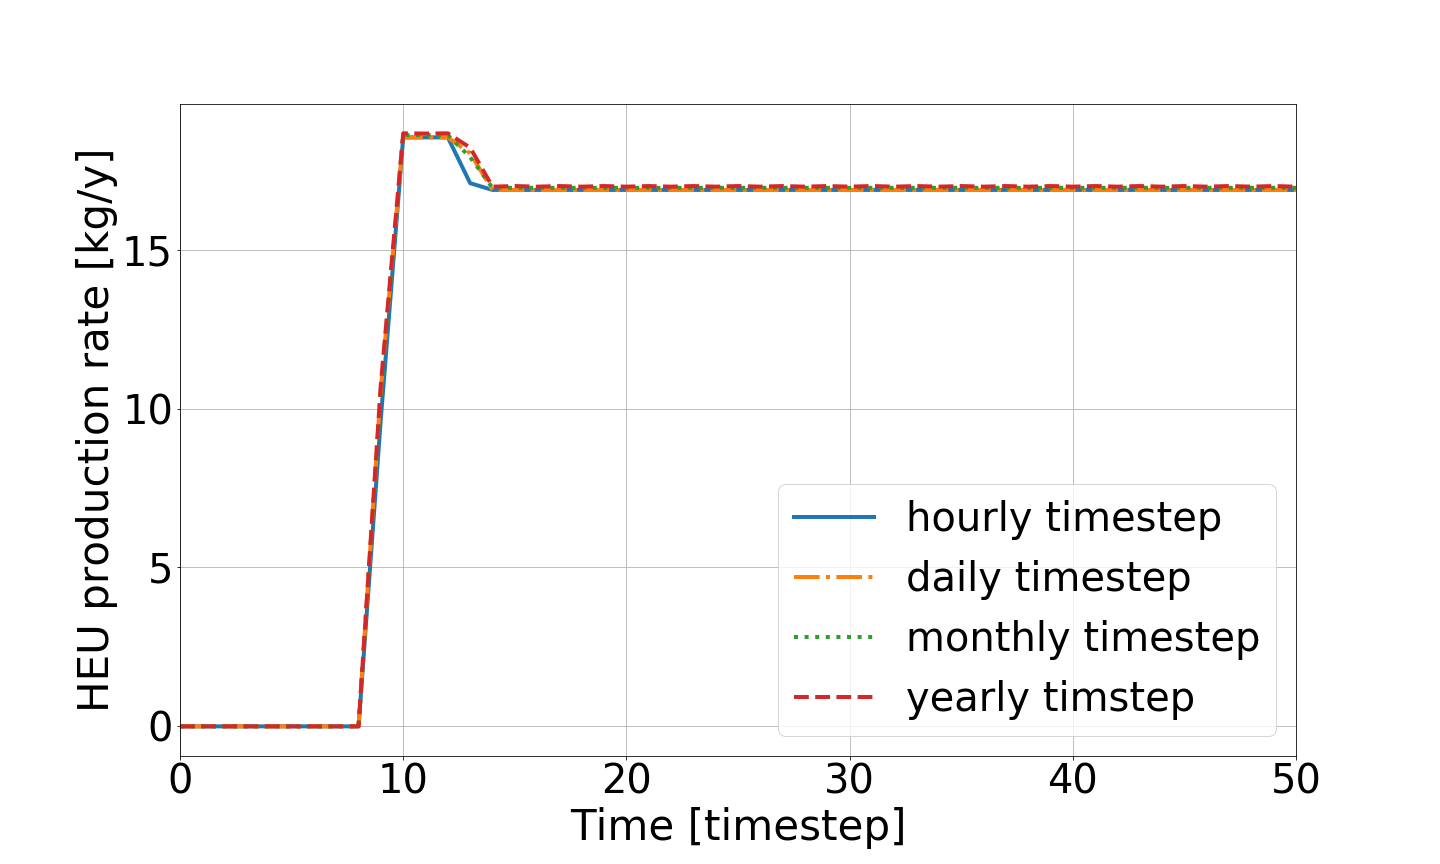
\includegraphics[scale=0.18]{HEU_prod_timestep}
%%     \caption{}
%%     \label{fig:HEU_timestep}
%% \end{figure}

\begin{figure}[t!]
    \centering
    \begin{subfigure}[t]{0.45\textwidth}
        \centering
        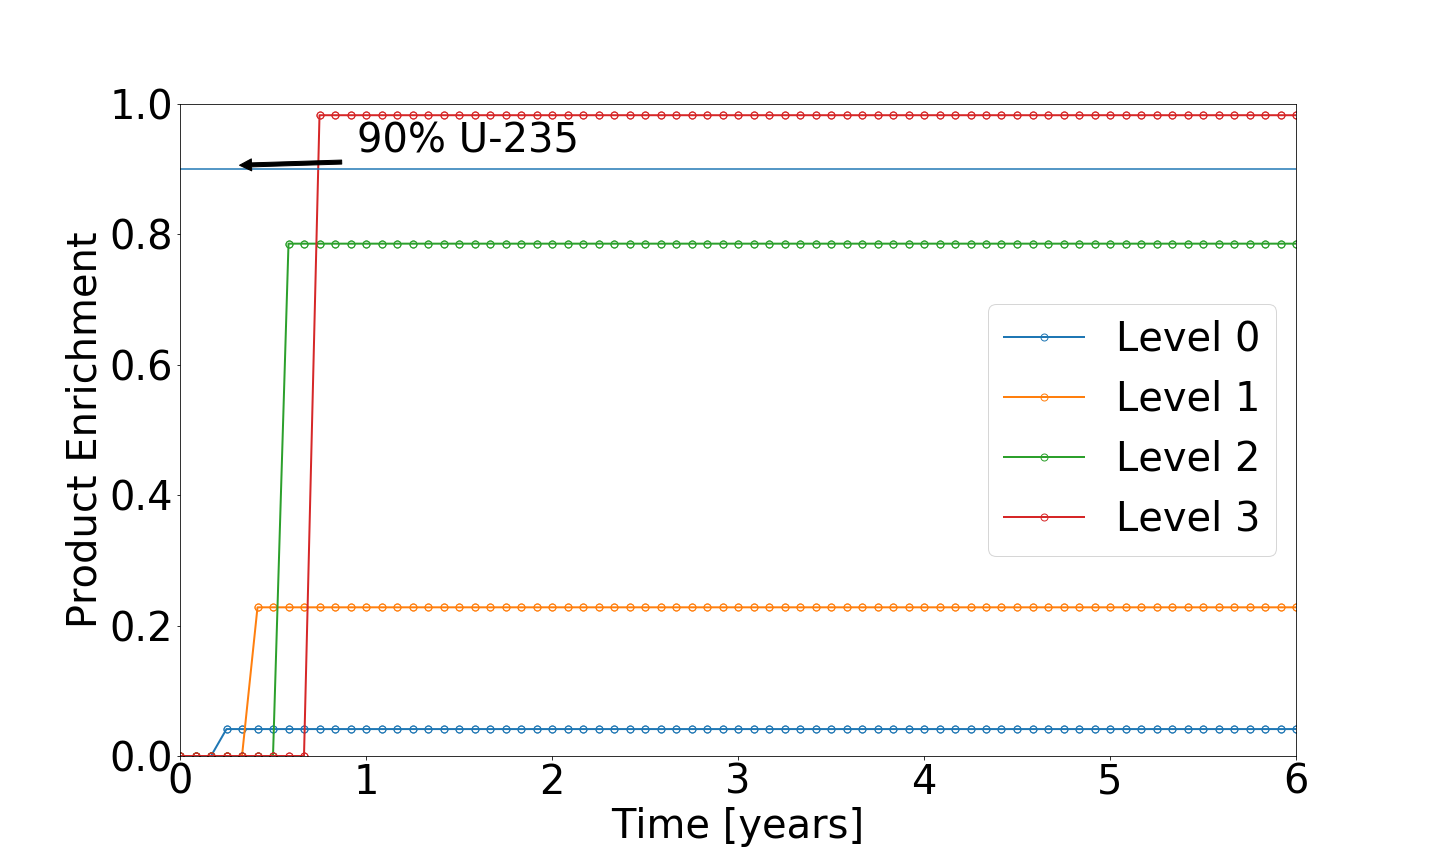
\includegraphics[scale=0.18]{NR_case1}
        \caption{No tail recycling}
    \end{subfigure}%
    \begin{subfigure}[t]{0.45\textwidth}
        \centering
        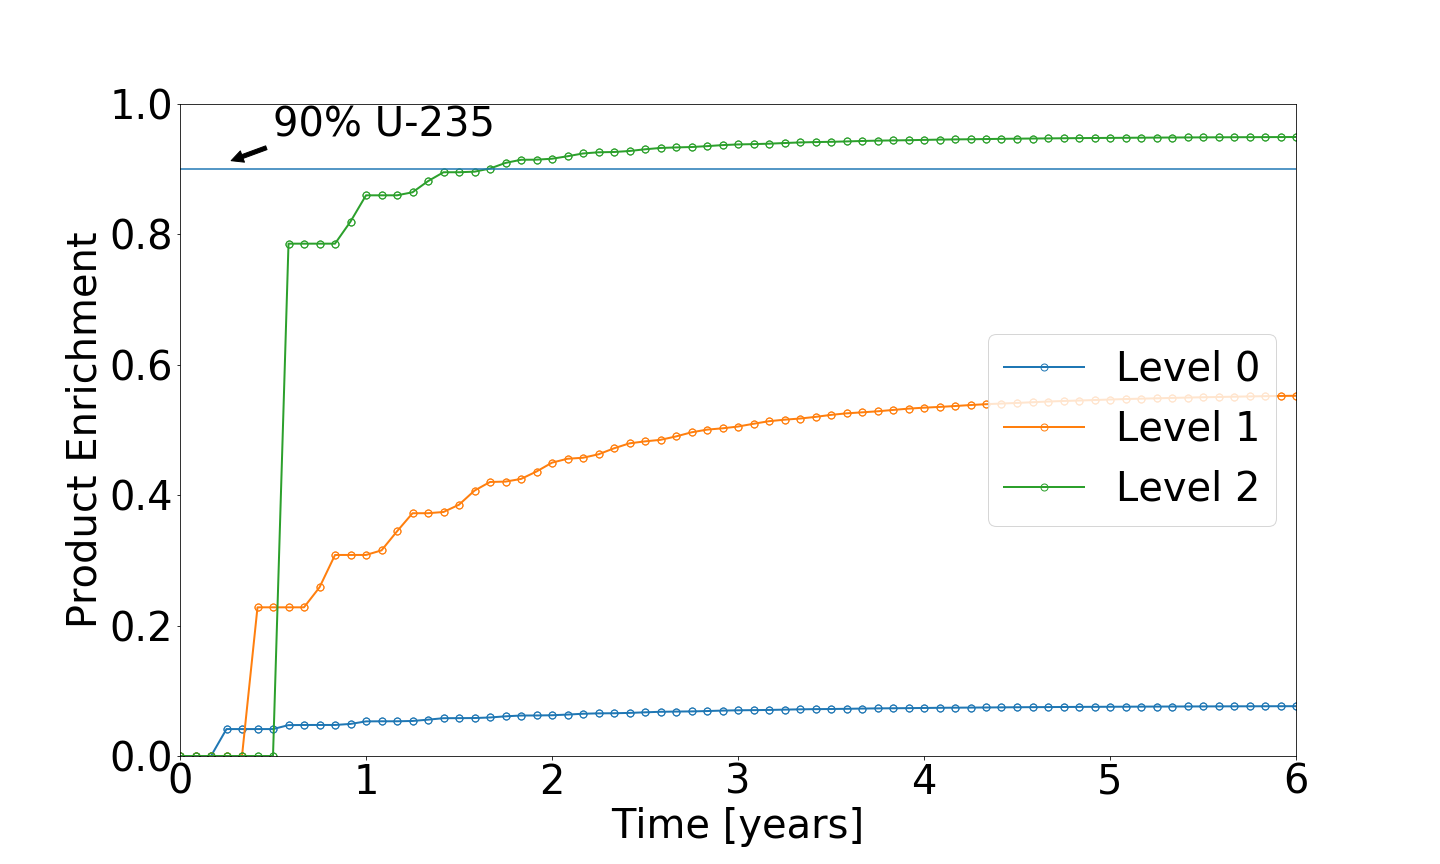
\includegraphics[scale=0.18]{R_case1}
        \caption{Tail recycling}
    \end{subfigure}
    \caption{Evolution of the product assays at each level with considering
    miss-use model A, with (right) and without recycling (left).}
\end{figure}
\begin{figure}[t!]
    \centering
    \begin{subfigure}[t]{0.45\textwidth}
        \centering
        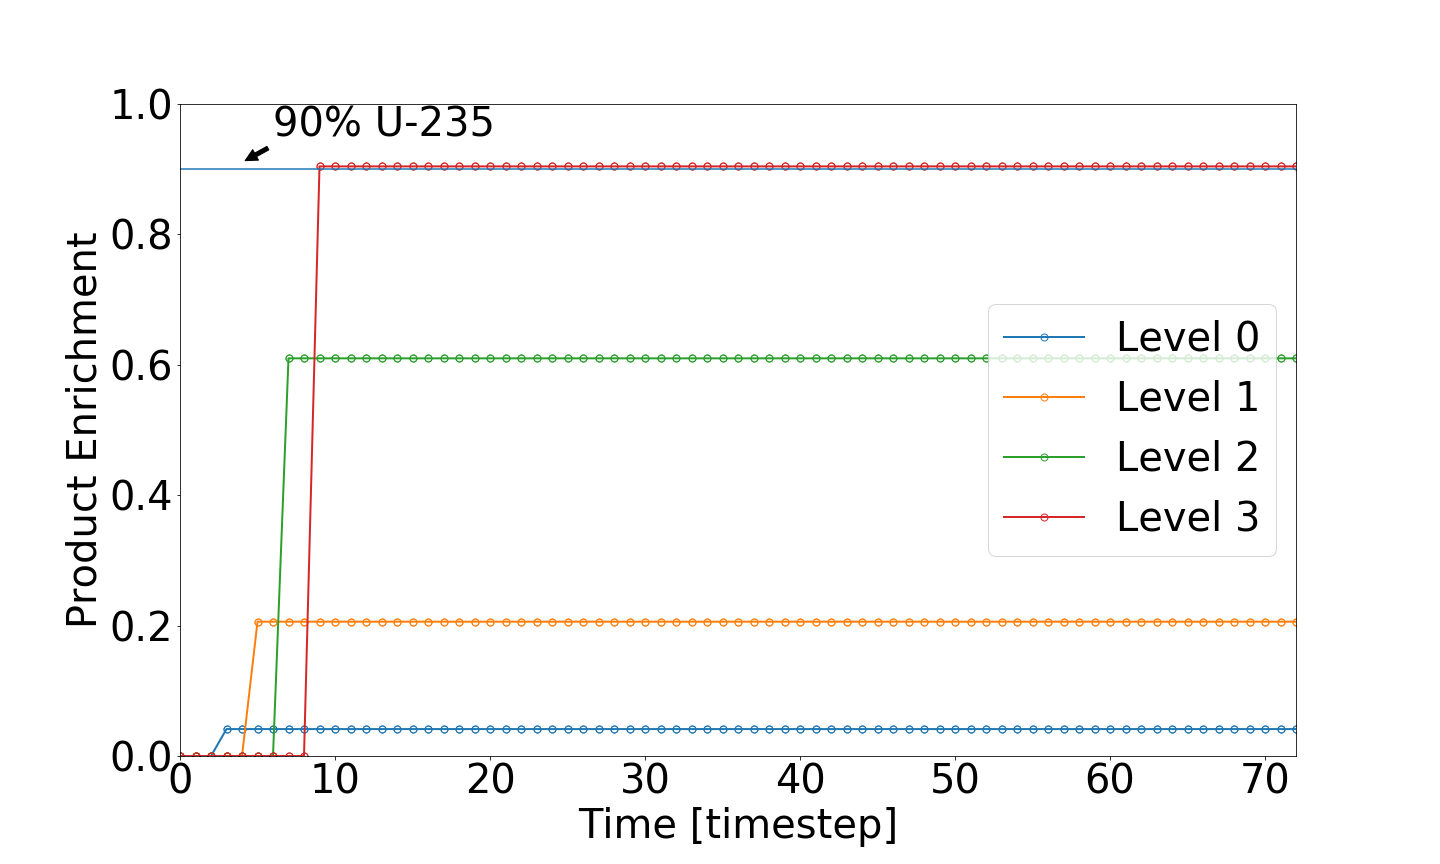
\includegraphics[scale=0.18]{NR_case2}
        \caption{No tail recycling}
    \end{subfigure}%
    \begin{subfigure}[t]{0.45\textwidth}
        \centering
        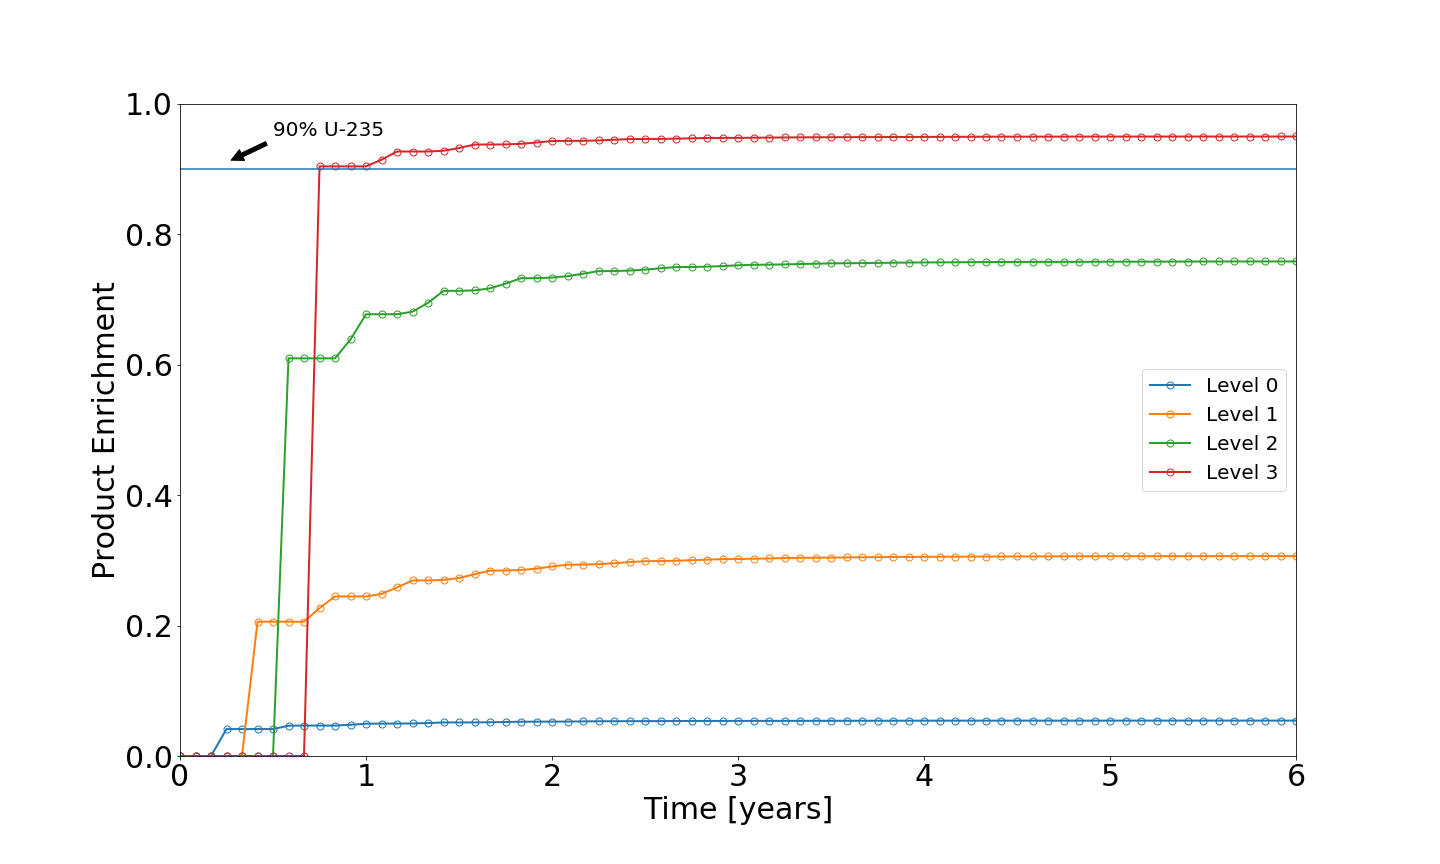
\includegraphics[scale=0.18]{R_case2}
        \caption{Tail recycling}
    \end{subfigure}
    \caption{Evolution of the product assays at each level with considering
    miss-use model B, with (right) and without recycling (left).}
\end{figure}
\begin{figure}[t!]
    \centering
    \begin{subfigure}[t]{0.45\textwidth}
        \centering
        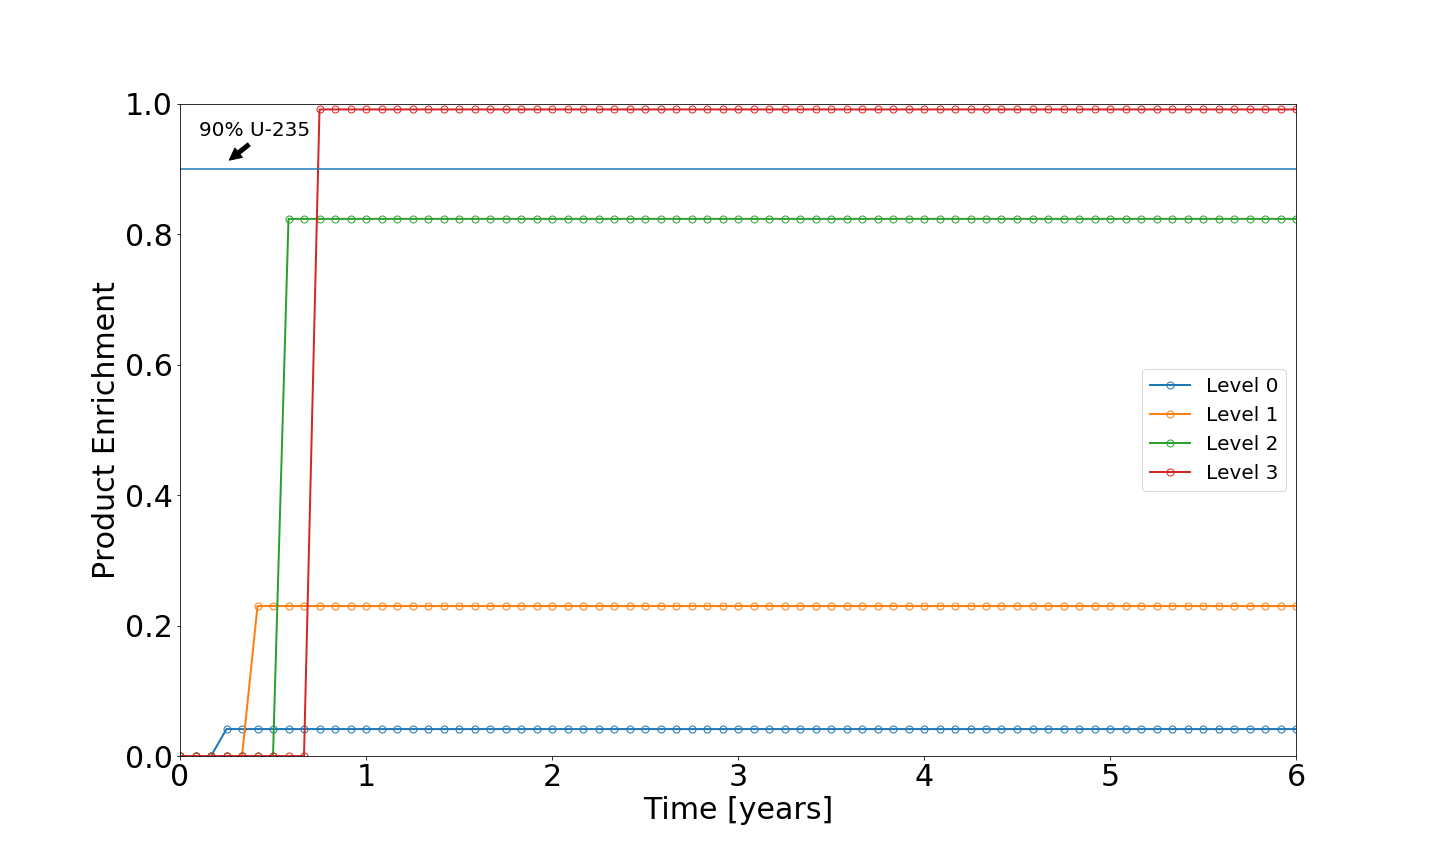
\includegraphics[scale=0.18]{NR_case3}
        \caption{No tail recycling}
    \end{subfigure}%
    \begin{subfigure}[t]{0.45\textwidth}
        \centering
        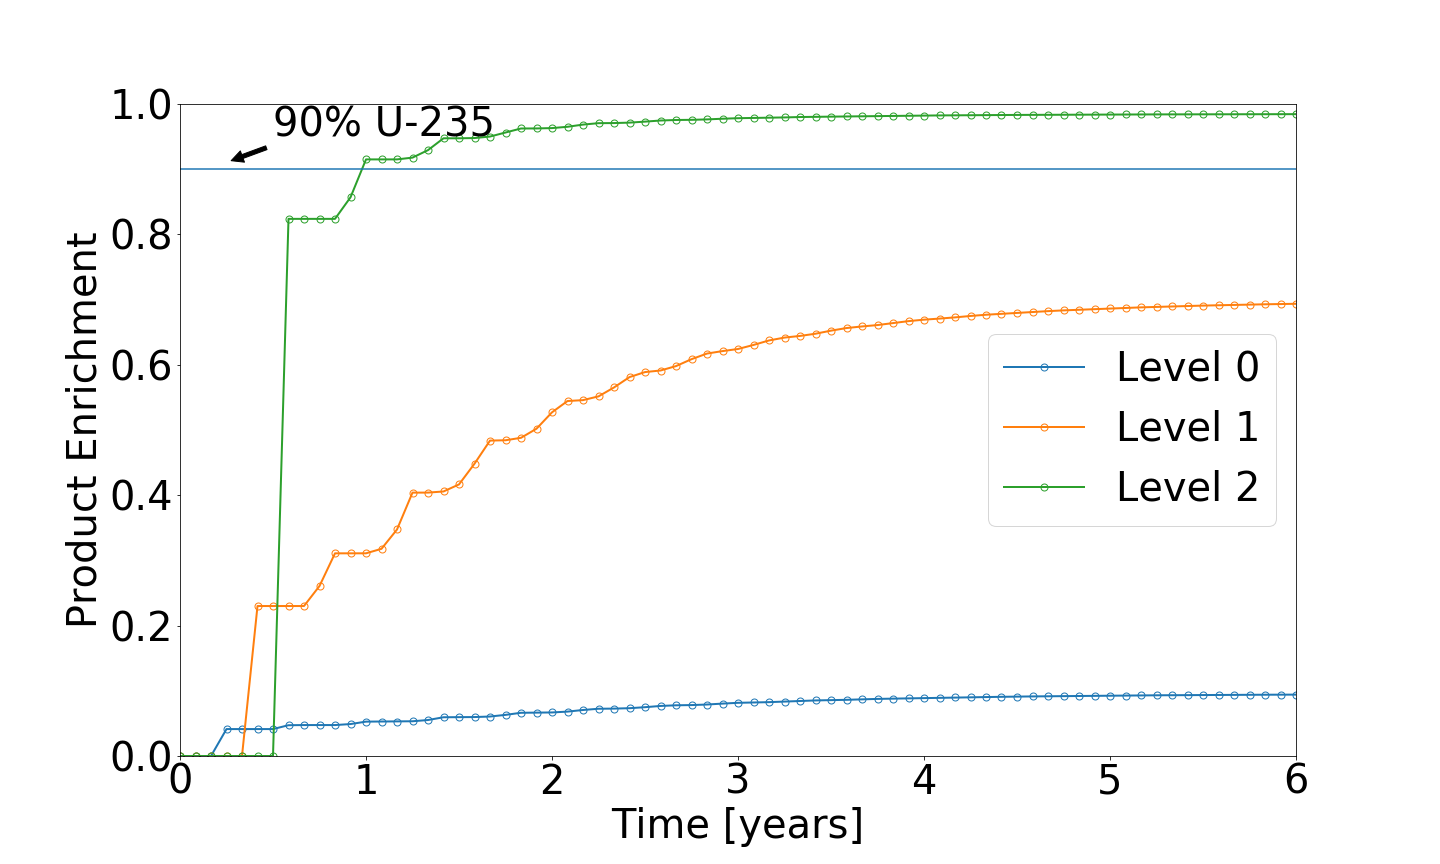
\includegraphics[scale=0.18]{R_case3}
        \caption{Tail recycling}
    \end{subfigure}
    \caption{Evolution of the product assays at each level with considering
    miss-use model C, with (right) and without recycling (left).}
\end{figure}

\begin{figure}[ht] % replace 't' with 'b' to force it to be on the bottom
    \centering
    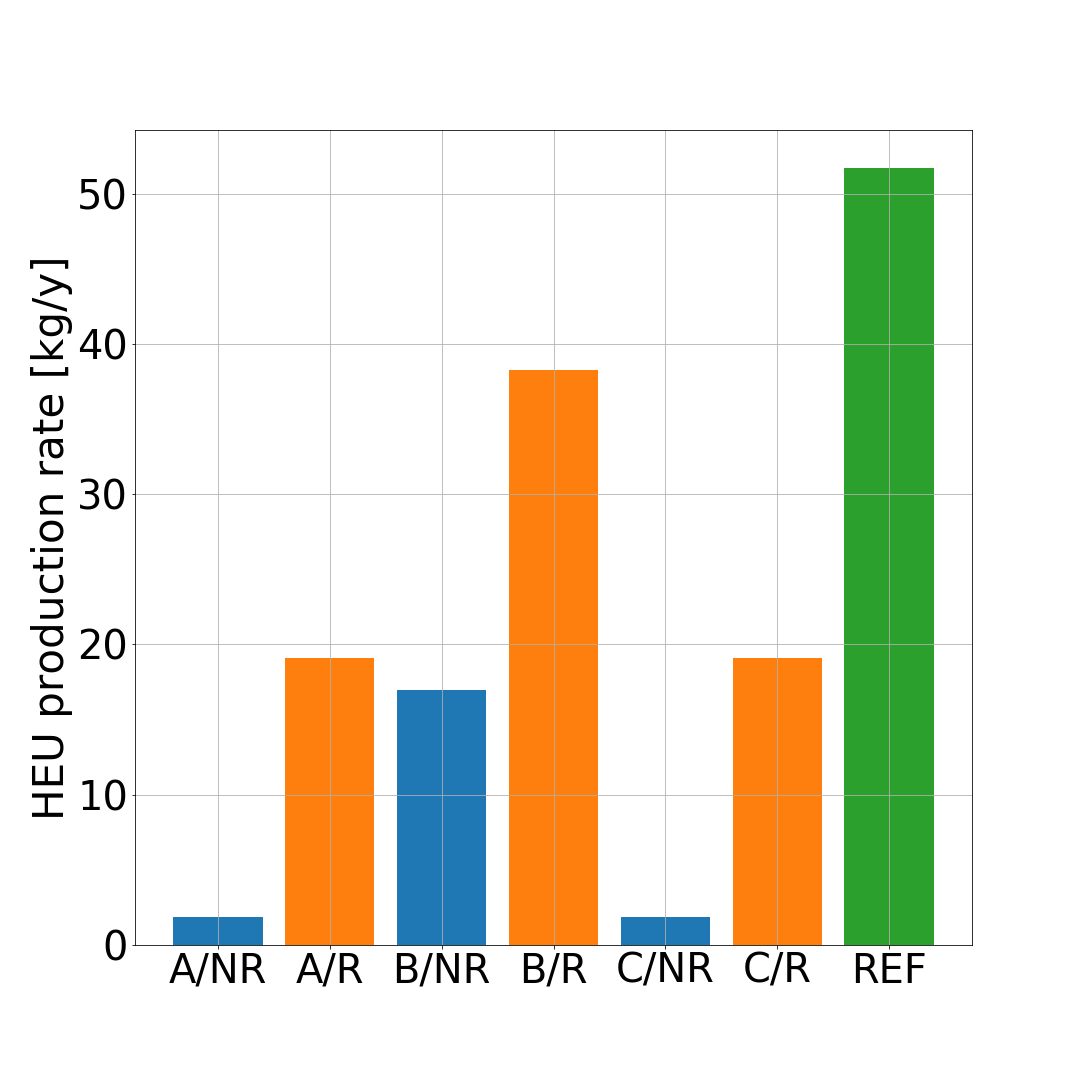
\includegraphics[scale=0.25]{HEU_prod_rate}
    \caption{Production rate for the different model configuration, with in blue
    the case without tail recycling, in orange with tail recycling, and in green
    the reference one.}
    \label{fig:HEU_rate}
\end{figure}
